\chapter{Avaliação da plataforma}

Nesse capítulo apresentamos um exemplo do uso do Comunidade.UnB em um ambiente
universitário e uma pesquisa com os alunos que fizeram uso do mesmo.
%
O estudo de caso foi baseado no uso do Comunidade.UnB, de diferentes formas em
três disciplinas do curso de Engenharia de Software da FGA:
%
Desenho Industrial Assistido po Computador~\footnote{\url{%
https://wwwsec.serverweb.unb.br/matriculaweb/graduacao/disciplina.aspx?cod=199176}} (DIAC), 1º semestre;
%
Orientação a Objetos~\footnote{\url{%
https://wwwsec.serverweb.unb.br/matriculaweb/graduacao/disciplina.aspx?cod=195341}}
(OO), 3º semestre;
%
Manutenção e Evolução de Software~\footnote{\url{
https://wwwsec.serverweb.unb.br/matriculaweb/graduacao/disciplina.aspx?cod=206598}}
(MES), 7º semestre;
%
com a criação de uma comunidade para cada uma das disciplinas. Para a disciplina de
MES foram usadas ainda sub-comunidades para cada um dos projetos trabalhados nela.

\section{Uso do Noosfero em Disciplinas do Curso de Engenharia de Software}
\label{mes-unb}

O nível de uso da ferramenta variou de acordo com o semestre da disciplina. Na
disciplina de DIAC a comunidade foi utilizada mais como uma fonte de notícias
partindo do professor para os alunos. Os alunos foram encorajados ainda a publicar
as imagens de seus desenhos nas galerias de imagens de seus perfis, conforme
visto na Figura \ref{imagem-diac}.

\begin{figure}[h!]
    \centering
		\rule{1cm}{1cm}
    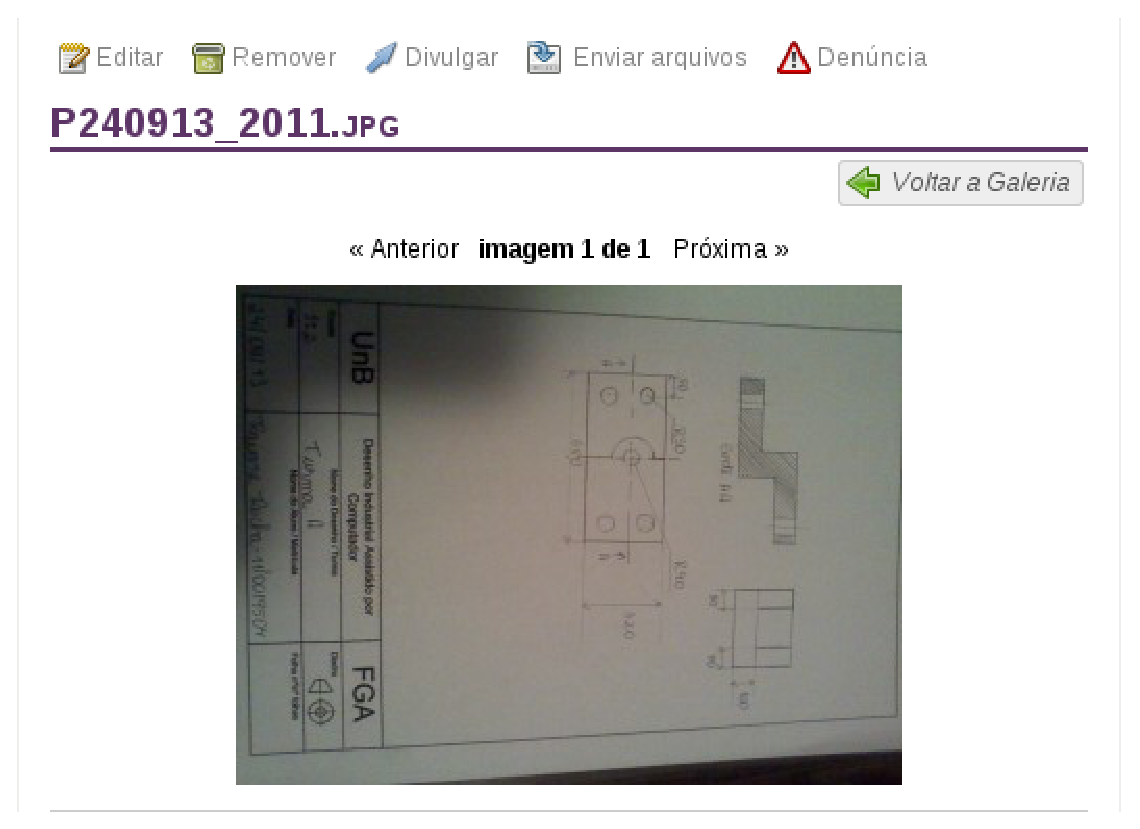
\includegraphics[keepaspectratio=true,scale=0.65]
      {figuras/imagem-diac.eps}
    \caption{Desenho desenvolvido na disciplina de DIAC:\newline
\url{http://comunidade.unb.br/raiane/galeria/p240913-2011.jpg}}
    \label{imagem-diac}
\end{figure}

A comunidade da disciplina de OO foi utilizada para  publicar os enunciados dos
trabalhos da disciplina e para receber os trabalhos dos alunos. Os enunciados
das provas das disciplinas também foram publicados na comunidade, assim como
seus gabaritos e revisões.
%
Na disciplina de MES, os alunos foram divididos em grupos para trabalhar com
manutenção e evolução de três projetos de software livre. Para isso foram
criadas sub-comunidades para cada um dos projetos:
%
(\textit{i}) Analizo;
(\textit{ii}) Noosfero;
e (\textit{iii}) Radar Parlamentar;
%
de forma que os progressos alcançados, materiais de estudo, referências
bibliográficas etc fossem publicadas em suas próprias sub-comunidades%
~\footnote{Uma sub-comunidade funciona como uma comunidade comum, porém
associada ao a uma comunidade ``mãe''.} (através do \textit{plugin} de
sub-organizações).

\begin{figure}[h!]
    \centering
    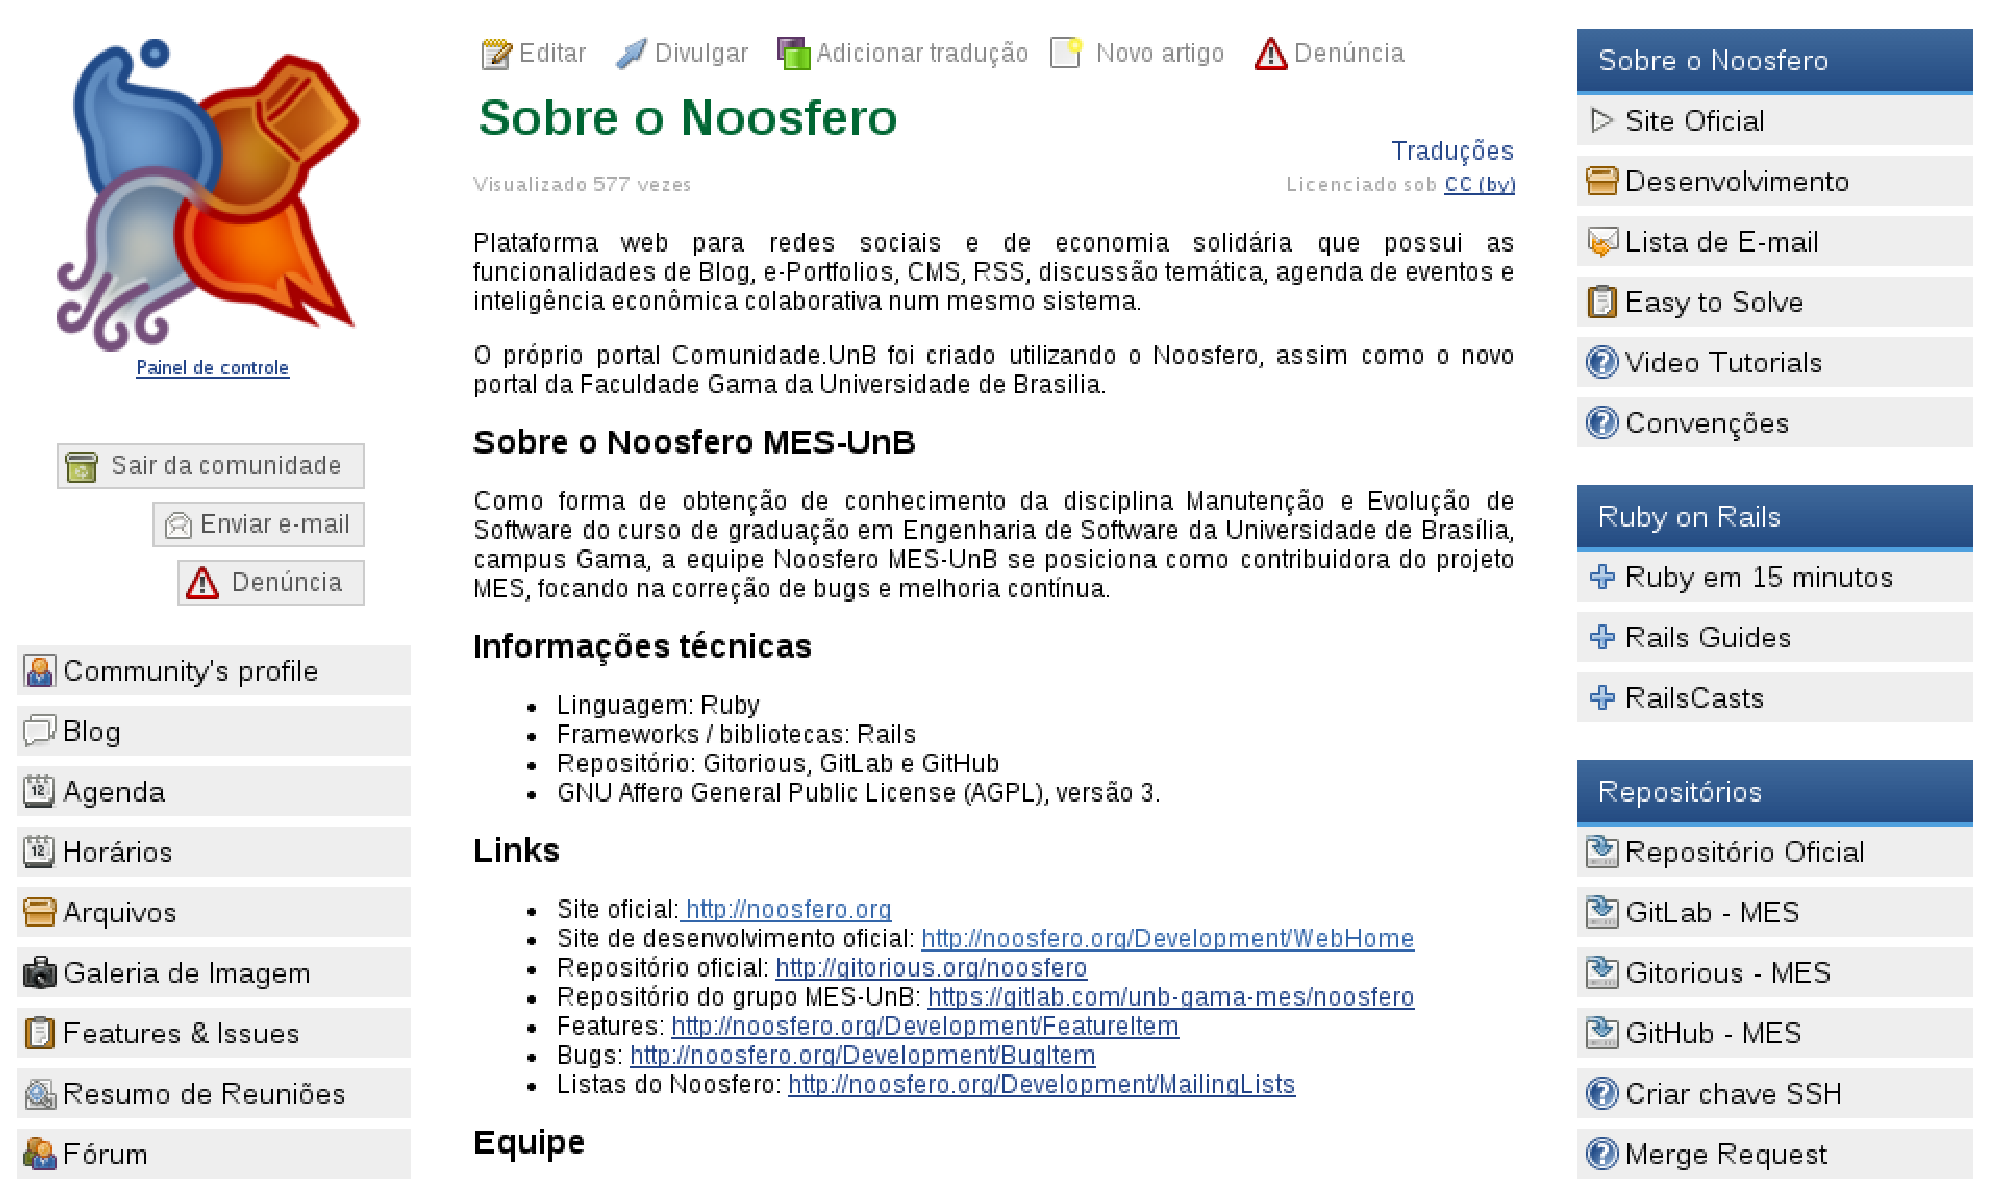
\includegraphics[keepaspectratio=true,scale=0.35]
      {figuras/Noosfero-MES.eps}
    \caption{Página inicial da sub-comunidade do projeto Noosfero da disciplina
    de MES:\newline \url{http://comunidade.unb.br/noosfero-mes-fga}}
    \label{mes-noosfero}
\end{figure}

A Figura \ref{mes-noosfero} apresenta a página inicial,  da sub-comunidade do
time que colaborou com o Noosfero. Notamos que, conforme aumentava o semestre da
disciplina, e consequentemente a maturidade intelectual de seus alunos, o nível
do uso das funcionalidades de CMS do Noosfero, como a adição de blocos
laterais personalizados e a criação de conteúdos diversos, aumentou.

\section{Pesquisa com os usuários}

No mês de Dezembro de 2013, realizamos uma pesquisa junto aos alunos das três
disciplinas sobre o uso de uma rede social associada à marca da universidade
e sobre o nível de adequação do Noosfero para ser a plataforma adotada para
implantar essa rede.
%
Foi criado um questionário com cinco questões objetivas, com a opção de
justificativa para as respostas.
%
Nesta seção, apresentamos as questões elaboradas e as respostas coletadas
através da ferramenta \textit{Google Drive}. Foram coletadas, ao todo,
34 respostas (voluntárias) ao questionário, de um total possível de 88 alunos
das três turmas.

\subsection*{Questão preliminar: Qual o seu semestre?}

\begin{figure}[h!]
    \centering
    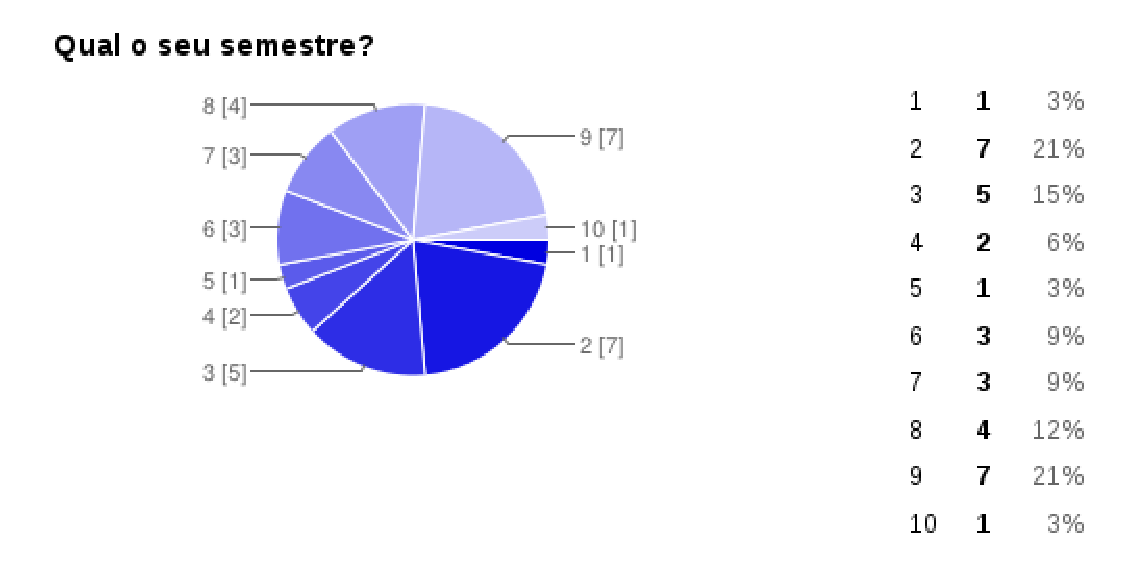
\includegraphics[keepaspectratio=true,scale=0.6]
      {figuras/p0.eps}
    \caption{Gráfico de respostas à questão preliminar.}
    \label{response:0}
\end{figure}

A primeira pergunta tinha como objetivo levantar qual o semestre dos alunos
a responder o questionário e assim possivelmente associar as respostas
ao nível de maturidade dos alunos e ao tipo de uso que estes fizeram da rede.
%
A Figura \ref{response:p0} apresenta o resultado das pergutas. Podemos perceber
que a distribuição dos alunos teve maior peso nos semestres iniciais,
principalmente do segundo e terceiro, e nos semestres finais, com alunos
do oitavo e nono semestres.

\subsection*{Questão 01: Você vê utilidade na possibilidade de uma rede social
com foco na colaboração e construção de conhecimento para uma universidade?}

\begin{figure}[h!]
    \centering
    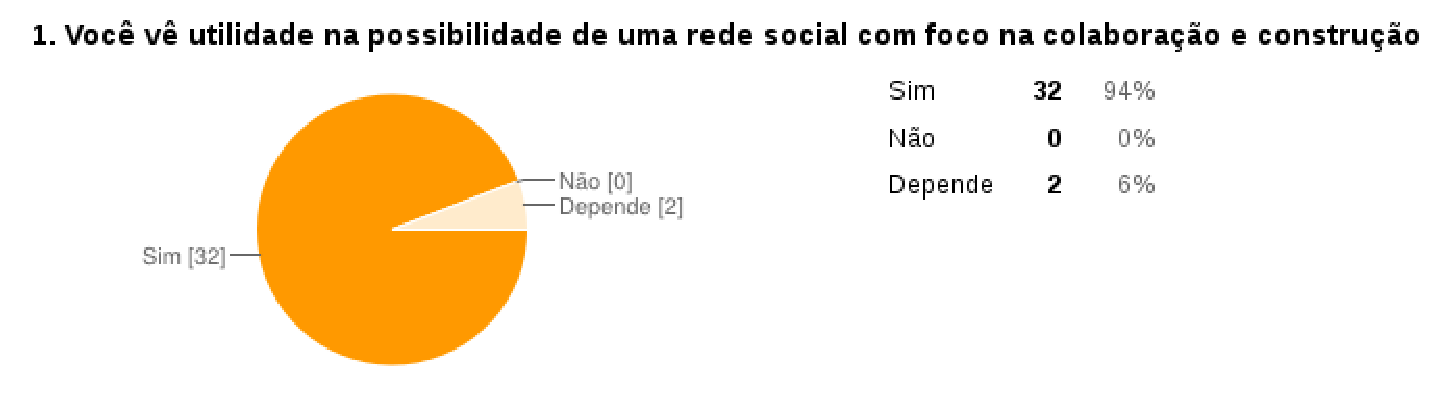
\includegraphics[keepaspectratio=true,scale=0.55]
      {figuras/p1.eps}
    \caption{Gráfico de respostas à questão 01.}
    \label{response:1}
\end{figure}

Podemos notar que 32 dos 34 (94\%) alunos que responderam ao questionário, responderam
que vêm utilidade em uma rede de colaboração para a universidade, e outros dois alunos
responderam que talvez (Figura \ref{response:1}).
%
Entre as justificativas, os alunos escreveram coisas como:

\begin{center}
``\textit{A vida acadêmica fica muito mais integrada com a colaboração em grupo.}'';
\end{center}

e

\begin{center}
``\textit{Atualmente é de extrema importância o desenvolvimento de atividades
em grupo que permitem atingirmos o objetivo de maneira mais natural e com menor
sobrecarga.}''.
\end{center}

\subsection*{Questão 02: Você utilizaria uma rede social de sua universidade na
qual todo o conteúdo produzido é associado à marca da universidade?}

\begin{figure}[h!]
    \centering
    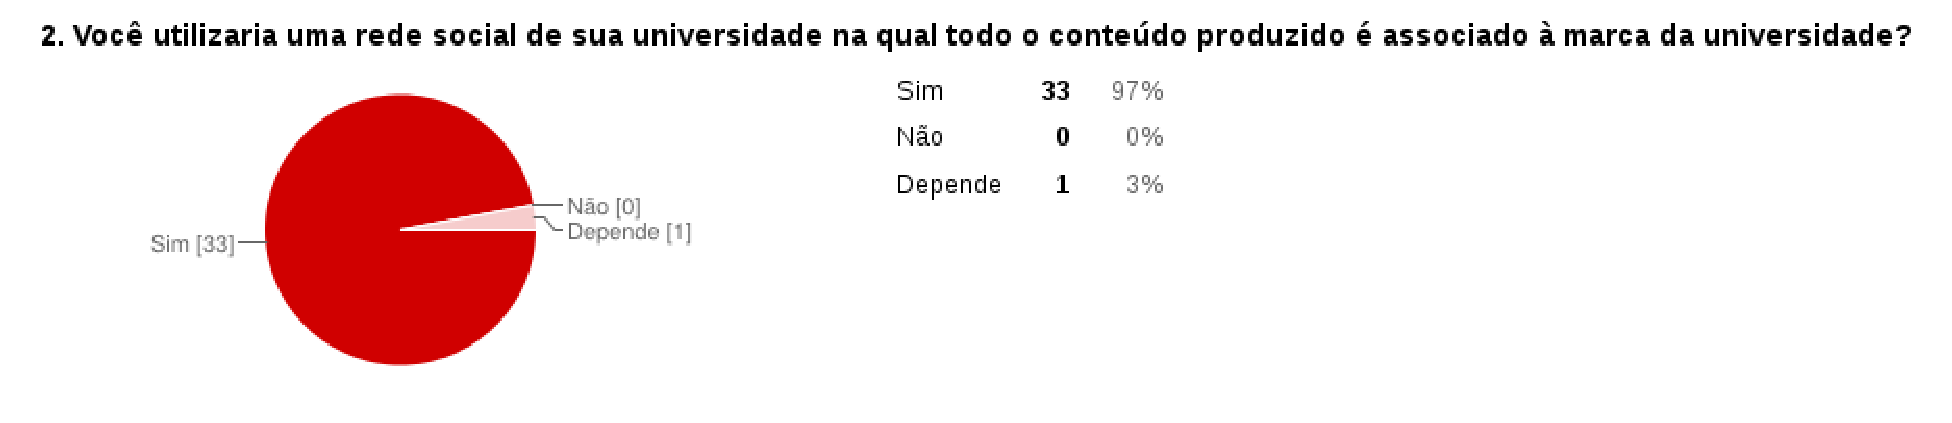
\includegraphics[keepaspectratio=true,scale=0.55]
      {figuras/p2.eps}
    \caption{Gráfico de respostas à questão 02.}
    \label{response:2}
\end{figure}

O intuíto desta questão foi averiguar se averia adesão à rede proposta. A Figura
\ref{response:2} apresenta os resultados obtidos e percebemos que, dos alunos que
tiveram contato com o Comunidade.UnB, nenhum declarou que não usaria, com 97\%
respondendo que sim e 3\% que talvez.

\subsection*{Questão 03: Que tipo de uso você faria/gostaria de fazer de uma
rede deste tipo?}

\begin{figure}[h!]
    \centering
    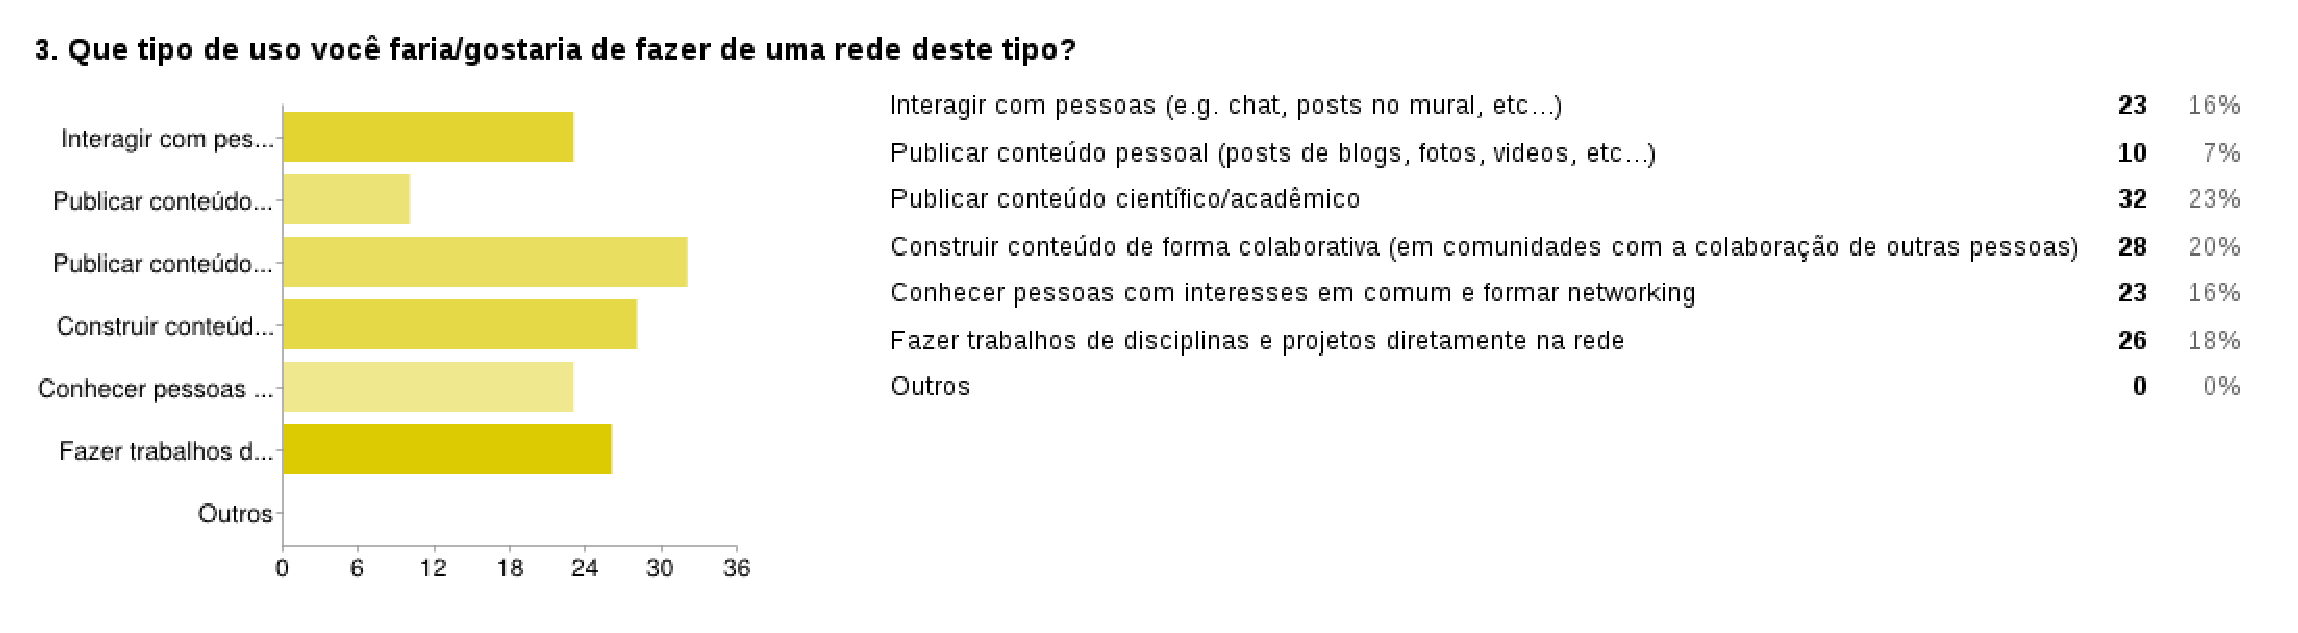
\includegraphics[keepaspectratio=true,scale=0.5]
      {figuras/p3.eps}
    \caption{Gráfico de respostas à questão 03.}
    \label{response:3}
\end{figure}

Analizando a Figura \ref{response:3}, percebemos que o interesse maior dos
alunos em uma rede como a proposta é a publicação e construção de conteúdo
científico/acadêmico, além da construção de \textit{networking} (rede de
relacionamento) acadêmico. Apenas 10 alunos responderam que utilizariam a rede
para publicar conteúdo pessoa.

\subsection*{Questão 04: Como você avalia o Noosfero para satisfazer as
necessidades de uma rede de colaboração para a UnB?}

\begin{figure}[h!]
    \centering
    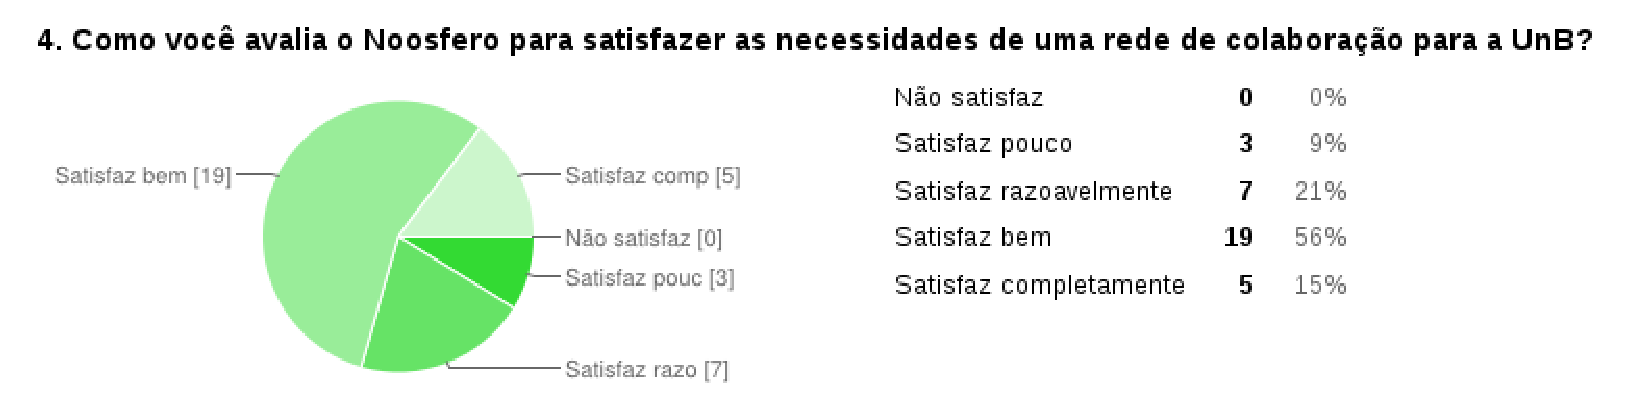
\includegraphics[keepaspectratio=true,scale=0.55]
      {figuras/p4.eps}
    \caption{Gráfico de respostas à questão 04.}
    \label{response:4}
\end{figure}

O objetivo dessa questão foi coletar a opinião dos alunos após um semestre de
contato com o Noosfero para saber se eles acham que este pode ser a plataforma
utilizada para a construção da rede de colaboração da UnB. Na Figura
\ref{response:4} percebemos que a maioria acha que sim, com 71\% respondendo
que o Noosfero satisfaz bem ou completamente. Nenhum dos entrevistados
respondeu que não satisfaz.
%
Entre os que responderam que não acham que o Noosfero satisfaz completamente,
as principais críticas foram em relação a usabilidade. Coletamos respostas
como:

\begin{center}
``\textit{Melhor usabilidade e look\&feel responsivo. Seria bom também ter os
recursos dos similares.}'';
\end{center}

e

\begin{center}
``\textit{Tem algumas funcionalidades que deveriam ser revista, levando em
consideracao a usablidade.}''.
\end{center}

Outra crítica foi em relação ao tipo de interação mais comum no Noosfero,
uma interação focada em comunidade. Um aluno respondeu que:

\begin{center}
``\textit{O Noosfero deveria focar um pouco mais na interação fora de
comunidades e focar um pouco na interação usuário-usuário.}''.
\end{center}

%-----------------------------------------------------------------------------%

Dentro a população que tivemos, alunos que estavam usando continuamente o
Noosfero desde Agosto de 2013, a amostra coletada nos proporcionou uma melhor
confirmação de nossas ideias ao propor a implantação de uma rede social de
colaboração na UnB.
%
No total, de forma voluntária, 34 alunos responderam ao questionário. Para as
respostas serem mais naturais, ou seja, sem a interferência do professor Paulo
Meirelles em sala de aula, apenas enviamos por e-mail o formulário de pesquisa,
para cerca de 88 alunos que fizeram, até o fim do semestre, uso do Noosfero
nas disciplinas mencionadas.
%
Os e-mails foram enviados aos alunos através da própria plataforma.

Ao analisar as respostas, percebemos que à proposta de uma rede, no moldes
abordados neste trabalho, foi aceito pelos alunos que tiveram tal experiência.
%
A maioria dos alunos avalia que o Noosfero pode ser a plataforma
utilizada para o Comunidade.UnB.
%
No próximo capítulo, ao concluir este relatório de trabalho de conclusão de curso,
propomos uma série de funcionalidades que julgamos agregadoras de valor ao
Noosfero, mas que não foi possível implementar durante a
execução deste trabalho, em 2013.
%
Entretanto, por outro lado, este trabalhou deixou, também, um legado humano,
através do conhecimento repassao à equipe do portal da UnB Gama (5 pessoas), que
implementarão tais funcionalidades em 2014.
%
Por fim, dentro dos trabalhos futuros, apresentaremos um primeiro levantamento
sobre a federação tecnológica, para prover a ``rede de redes'', um assunto
bastante debatido na comunidade do Noosfero.
